
\documentclass{jtetiproposalskripsi}

%-----------------------------------------------------------------
%Disini awal masukan untuk data proposal skripsi
%-----------------------------------------------------------------
\titleind{SISTEM INFORMASI PENDATAAN INVENTARIS PADA MADRASAH TSANAWIYAH NEGERI KENCONG}
\fullname{M. RIZAL FAHMI}

\idnum{1200631023}

\approvaldate{13 Februari 2015}

\degree{Sarjana Teknik Elektro}

\yearsubmit{2015}

\program{Manajemen Informatika}

\headprogram{Bagus Setya Rintyarna, S.T, M. Kom}

\firstsupervisor{Triawan Adi Cahyanto, M. Kom}
\firstnip{12 03 719}

\secondsupervisor{Bagus Setya Rintyarna, S.T, M. Kom}
\secondnip{09 03 521}


%-----------------------------------------------------------------
%Disini akhir masukan untuk data proposal skripsi
%-----------------------------------------------------------------

\begin{document}

\cover

\approvalpage

%-----------------------------------------------------------------
%Disini akhir masukan untuk muka skripsi
%-----------------------------------------------------------------

%-----------------------------------------------------------------
%Disini awal masukan Intisari
%-----------------------------------------------------------------
\begin{abstractind}
Inventaris merupakan daftar yang memuat semua barang milik kantor yang dipakai untuk melaksanakan tugas. Inventaris kantor sangatlah penting bagi kelangsungan sebuah Perusahaan maupun Instansi. Khususnya untuk Madrasah Tsanawiyah Negeri Kencong sistem pendataan dan pencatatan inventaris  yang digunakan selama ini masih menggunakan aplikasi pengolahan data secara manual yakni menggunakan tulisan tangan di dalam pembukuan. Hal dinilai kurang begitu efektif dan efisien dalam menunjang operasional madrasah. Ditambah dengan adanya mekanisme persutujuan (approval) ke Kepala Madrasah masih menggunakan nota tertulis sehingga akan sangat memerlukan waktu yang tidak sedikit mengingat jumlah inventaris yang cukup banyak.
\paragraph{}
Dari permasalahan tersebut memunculkan gagasan untuk membuat suatu aplikasi berbasis web, yang di dalamnya dapat melakukan pengelolaan dan pendataan inventaris madrasah. Metodologi yang digunakan dalam pembuatan aplikasi ini adalah metode Waterfall. Bahasa pemrogramannya adalah PHP dan HTML. Untuk tampilan menggunakan CSS3 dan Jquery. Databasenya menggunakan MySQL. Tools dan Editor yang digunakan ialah XAMPP for Windows versi 7.7, Photoshop, Macromedia dreamwaver CS3 .
\paragraph{}
Didukung dengan tersedianya jaringan internet lokal (LAN) di dalam Madrasah. Aplikasi ini nantinya akan digunakan sebagai media pendataan serta pengontrol inventaris, pendataan inventaris dilakukan oleh staff admin. Dengan adanya Aplikasi Manajemen Inventaris Madrasah Berbasis Web ini diharapkan akan mempermudah administrator dalam mengelola inventaris – inventaris Madrasah  sehingga hasil pelaporan data dapat diketahui dengan mudah, cepat dan akurat.



\bigskip
\textbf{Kata kunci} : Inventaris, Madrasah, Metode Waterfall, Staff admin.
\end{abstractind}
%-----------------------------------------------------------------
%Disini akhir masukan Intisari
%-----------------------------------------------------------------

\tableofcontents
\listoftables
\listoffigures
\addcontentsline{toc}{chapter}{DAFTAR ISI}
\selectlanguage{bahasa}\clearpage\pagenumbering{arabic}\setcounter{page}{1}




%-----------------------------------------------------------------
%Disini awal masukan untuk Bab
%-----------------------------------------------------------------
\chapter{LATAR BELAKANG}

\section{Latar Belakang Masalah}
Madrasah Tsanawiyah Negeri Kencong berlokasi di Desa Wonorejo Kecamatan Kecong Kabupaten Jember. Madrasah Tsanawiyah Negeri Kencong sangat membutuhkan sistem informasi dalam pendataan inventaris barang Madrasah . 
\paragraph{}
Saat ini Sistem pendataan inventaris Madrasah yang berjalan di Madrasah Tsanawiyah Ar-Rohman masih menggunkan sistem manual yaitu berupa tulisan tangan dalam pembukuan. Walaupun sempat didukung dengan komputer tetapi hanya memanfaatkan  Microsoft Office Standar (Microsoft Office Excel dan Word)  sehingga memungkinkan banyak sekali kesalahan dalam pendataan inventaris. Hal ini dapat mengakibatkan kesulitan dalam pencarian data dan menyita waktu dalam pembuatan laporan. 
\paragraph{}
Untuk membantu pendataan inventaris di Madrasah Tsanawiyah Negeri Kencong perlu adanya suatu sistem informasi agar setiap pekerjaan yang menyangkut pencatatatn inventaris tersebut dapat dikurangi tingkat kesalahannya serta dapat memberikan pelayanan yang memuaskan terhadap siswa.
\paragraph{}
Berdasarkan latar belakang ini maka penulis dalam proposal tugas ahir ini mengambil judul : 
”SISTEM INFORMASI PENDATAAN INVENTARIS PADA MADRASAH TSANAWIYAH NEGERI KENCONG”


\section{Rumusan Masalah}
Sesuai dengan latar belakang yang telah di uraikan diatas pada pembahasan latar belakang masalah, maka rumusan masalah yang akan di selesaikan adalah:
\begin{itemize}
\item[1.]Bagaimana merancang sistem pendataan inventaris pada Madrasah Tsanawiyah Negeri Kencong ?
\item[2.]Bagaimana membangun sebuah aplikasi sistem pendataan inventaris yang mampu mengelola dan mengolah data-data inventaris menjadi  suatu informasi yang dibutuhkan?
\end{itemize}

\section{Batasan Masalah}
Agar pembahasan masalah tidak menyimpang dari tujuan penelitian, maka berikut adalah batasan masalah pada  penelitian ini:
\begin{itemize}
\item[1.]Data inventaris yang dimaksud adalah data di MTs Negeri Kencong
\item[2.]Report yang ditampilan meliputi, cara peroleh, sumber dana, tahun, jenis barang, peminjaman, sehingga tidak membahas laporan lainnya.

\end{itemize}

\section{Maksud dan Tujuan}
Maksud dari penulis mengambil judul ini adalah :



\begin{itemize}
\item[1.]Untuk memenuhi salah satu syarat dalam menyelesaikan Program Studi Diploma III Jurusan Manajemen Informatika di Universitas Muhammadiyah Jember
\item[2.]Menciptakan sistem yang mampu menghasilkan informasi data Inventaris barang yang tersedia, juga untuk membuat suatu perancangan sistem baru yang mengolah data Inventaris barang dengan bantuan komputer  
\end{itemize}
Sedangkan tujuan dari Perancangan Sistem Informasi Sistem Informasi Inventaris di MTs Negeri Kencong adalah: 
\begin{itemize}
\item[1.]Memudahkan pengolahan dan penyajian data inventaris barang di MTs Negeri Kencong untuk kedepannya.
\item[2.]Mengkomputerisasi sistem informasi pendataan inventaris di MTs Negeri Kencong dalam pengolahan data siswa dengan mengembangkan sistem yang sudah ada menjadi lebih baik.
\end{itemize}


\section{Manfaat Penelitian}
Dengan adanya komputerisasi sistem informasi penerimaan siswa baru ini diharapkan dapat memberikan manfaat manfaat sebagai berikut :
\begin{itemize}
\item[1.]Menerapkan ilmu yang telah diperoleh selama kuliah di Universitas Muhammadiyah Jember 
\item[2.]Dapat merancang sebuah sistem yang profesional dan program yang bermanfaat bagi pihak MTs Negeri Kencong 
\item[3.]Dapat memberikan masukan terhadap operasional sistem pendataan Inventaris di  MTs Negeri Kencong.
\item[4.]Mengembangkan sistem yang sudah ada menjadi lebih baik
\end{itemize}

\section{Sistematika Penulisan}
Berikut sistematika penyusunan tugas akhir yang akan disusun :
\\
\textbf{BAB I     PENDAHULUAN}
\\
Pada bab ini memuat tentang latar belakang masalah, perumusan masalah, batasan masalah, tujuan dan manfaat penulisan, serta sistematika penulisan.
\\
\\
\textbf{BAB II    TINJAUAN KEPUSTAKAAN}
\\
Pada bab ini dibahas tentang gambaran umum instansi, mencakup sejarah dan struktur organisasi, kajian kepustakaan, mekanisme pengolahan data secara manual, landasan teori atau pun konsep yang berhubungan dengan sistem aplikasi berbasis Web.
\\
\\
\textbf{BAB III  METODE PENELITIAN}
\\
Dalam bab ini dibahas tentang metodelogi penelitian, tahapan pengumpulan databarang yang digunakan dalam analisa data.
\\
\\
\textbf{BAB IV  MEMBANGUN SISTEM APLIKASI DAN PEMBAHASAN}
\\
Pembahasan  pada  bab  ini  tentang  membangun  sistem  aplikasi  pencatatan inventaris meliputi diagram konteks, diagram fungsional dan flowcart sistem serta tampilan aplikasi pencatatan inventaris.
\\
\\
\textbf{BAB V    PENUTUP}
\\
Membahas tentang kesimpulan berdasarkan  pembahasan sebelumnya serta saran untuk pengembangan program, lembaga maupun untuk instansi. 



%-------------------------------------------------------------------------------
\chapter{TINJAUAN PUSTAKA DAN DASAR TEORI}                

\section{Tinjauan Umum Sistem Informasi}
\subsection{Sistem}
Menurut  (Davis, 1991:68) sebuah sistem terdiri dari bagian-bagian saling berkaitan yang beroperasi bersama untuk mencapai beberapa sasaran atau maksud. Suatu sistem adalah suatu jaringan kerja dari prosedur-prosedur yang saling berhubungan, berkumpul bersama-sama untuk melakukan suatu kegiatan atau untuk menyelesaikan suatu sasaran tertentu. Berarti, sebuah sistem bukanlah seperangkat unsur yang tersusun secara tak teratur, tetapi terdiri dari unsur yang dapat dikenal sebagai saling melengkapi karena satunya maksud, tujuan, atau sasaran. Jadi sistem adalah sekelompok elemen yang terintegrasi dengan maksud yang sama untuk mencapai suatu tujuan. Model umum sebuah sistem terdiri dari masukan, pengolah dan keluaran.

\subsection{Informasi}
Informasi menurut (Davis, 2003:28) merupakan data yang telah diolah menjadi sebuah bentuk yang berarti bagi penerimanya dan bermanfaat dalam pengambilan keputusan saat ini atau saat mendatang. Informasi yang baik adalah informasi yang mempunyai nilai kegunaan, tepat waktu, relevan, dan dapat dipercaya. Sumber dari informasi adalah data.
\\
Data menurut (Kadir, 2008:5) adalah deskripsi tentang benda, kejadian, aktivitas dan transaksi yang tidak mempunyai makna atau tidak berpengaruh secara langsung kepada pemakai. Jadi informasi dapat disimpulkan bahwa informasi bermuara pada data, memberikan nilai tambah atau pengetahuan bagi yang menggunakannya serta dapat digunakan untuk pengambilan keputusan. Informasi dalam lingkup sistem informasi menurut (Davis, 1991:29) memiliki beberapa ciri:
\begin{itemize}
\item[1.]Benar atau salah. Ini dapat berhubungan dengan realitas atau tidak. Bila penerimaan informasi yang salah mempercayainya, akibatnya sama seperti yang benar.
\item[2.]Baru, informasi dapat samasekali baru dan segar bagi penerimanya.
\item[3.]Tambahan, informasi dapat memperbarui atau memberikan tambahan baru pada informasi yang telah ada.
\item[4.]Korektif, informasi dapat menjadi suatu koreksi atau informasi salah atau palsu sebelumnya.
\end{itemize}

\paragraph{}
Seringkali dinyatakan bahwa informasi adalah hasil pemrosesan data. Prosesnya sendiri dapat berupa peringkasan, pererataan, penyajian, ke bentuk grafik, ataupun yang lain, dengan tujuan untuk memudahkan interpretasi manusia.

\subsection{Sistem Informasi}
Telah diketahi bahwa informasi merupakan hal yang sangat penting bagi manajemen didalam pengambilan keputusan. Sistem informasi didefinisikan oleh Robert A. Leitch dan K. Roscoe Davis (Rusmanto, 2011) sebagai suatu sistem didalam suatu organisasi yang mempertemukan kebutuhan pengolahan transaksi harian, mendukung operasi, bersifat manajerial dan kegiatan strategi dari suatu organisasi dan menyediakan pihak luar tertentu dengan laporan-laporan yang diperlukan. Sedangkan menurut Alter (Kadir, 2008:7) sistem informasi adalah kombinasi antara prosedur kerja, informasi, orang dan tekhnologi informasi yang diorganisasikan untuk mencapai tujuan dalam sebuah organisasi. Sistem informasi berarti sistem yang menggunakan teknologi informasi untuk menangkap, menyimpan, mengambil, menunjukkan suatu informasi yang digunakan suatu perusahaan atau lebih.


\section{Pengertian Database}
Merancang database merupakan hal yang sangat penting, kesulitan utama dalam merancang database adalah bagaimana merancang sehingga database dapat memuaskan keperluan dimasa mendatang.
\\
Menurut Budi (2004: 2) mengatakan bahwa database adalah sekumpulan data atau informasi yang terdiri atas satu atau lebih tabel yang saling berhubungan antara satu dengan yang  lainya.  Dan  kita  dapat  mengakses  data  tersebut,  baik  menambah,  mengganti, menghapus dan mengedit data dalam tabel tersebut.
\\
Definisi tentang database basis data mempunyai berbagai sumber data dalam pengumpulan data, bervariasi interaksi kejadian dari dunia nyata, dirancang dan di bangun agar dapat digunakan oleh beberapa pemakai untuk berbagai kepentingan.
\\
Database adalah kumpulan informasi yang disusun berdasarkan cara tertentu dan merupakan satu kesatuan yang utuh. Dengan sistem tersebut data yang dihimpun dalam suatu database dapat menghasilkan informasi yang berguna.
\\
Menurut Kadir (1999:9), basis data (database) secara umum  adalah kumpulan data, termasuk didalamnya adalah arsip-arsip berupa dokumen. Istilah basis data banyak menimbulkan interpretasi yang berbeda. Pada saat maraknya perangkat lunak dbase   dan dbase  plus, sebuah berkas (ekstensi.DBF) biasa disebut basis data. Istilah yang tidak tepat ini, meskipun telah masuk ke sejumlah pemogram, akhirnya diluruskan kembali oleh Febbri dan Schab, basis data adalah sistem berkas terpadu dirancang terutama untuk meminimalkan pengulangan data.
\\
Karakteristik dari database adalah :
\begin{itemize}
\item[a.]Database dipakai untuk mempresentasikan aspek-aspek dalam dunia nyata 
\item[b.]Database memiliki sekumpulan data teratur dan memiliki arti jelas
\item[c.]Database didesain, dibuat dan diisi dengan data untuk suatu tujuan tertentu dan pemakai tertentu. 
\end{itemize}

Beberapa istilah dalam database, yaitu :
\begin{itemize}
\item[a.]\textit{Table} adalah yang digunakan untuk menyimpan data yang berhubungan. Suatu tabel memiliki beberapa record (baris), dimana tiap record dibagi menjadi beberapa field (kolom). Tiap baris memiliki jumlah kolom yang sama. 
\item[b.]\textit{Record} adalah isi dari tabel yang dikenal juga dengan istilah row. Suatu record berisi informasi tentang item tersebut.
\item[c.]\textit{Field}  dikenal  juga  dengan  istilah  kolom  atau  attribute.  Suatu  field  berisi  sebagian informasi suatu record.
\item[d.]\textit{Primary   key}   adalah   suatu   attribute   yang   bersifat   unique   yang   dipakai   untuk mendefinisikan suatu record kedalam tabel.
\item[e.]\textit{Foreign key} adalah primary key dari suatu tabel dipakai sebagai non primary key field dari tabel.
\end{itemize}


\section{Tahap Perancangan Database}
Database merupakan kumpulan dari data yang saling berhubungan satu dengan yang lainnya, tersimpan disimpanan luar computer dan digunakan perangkat lunak tertentu untuk memanipulasinya. (Jogiyanto,2005)
Perancangan database bertujuan menjamin semua info yang diperlukan dalam organisasi meniadakan rangkap data, mengushakan banyaknya relasi database tentunya memberikan alat  handal  dan  mempresentasikan  data  dan  mengoptimalkan  database.  Perancangan database ini dimaksudkan untuk mengetahui dan menentukan field-field apa saja yang akan dibutuhkan untuk membangun suatu table sebagai dasar pembuatan database.

\begin{itemize}
\item[a.]\textbf{Diagram Konteks}
\\
Diagram konteks yaitu diagram yang menunjukkan batas dan jangkauan dari system informasi yang dibuat. Merupakan gambaran system secara garis besar dan memperlihatkan kelompok sata input dan output. Diagram konteks menggambarkan keterkaitan aliran-aliran data antara system  dengan  bagian-bagian luar  (kesatuan luar).  Kesatuan  ini  merupakan sumber arus data atau tujuan data yang berhubngan dengan system informasi tersebut. Diagram konteks memberikan batasan yang jelas mengenai besara-besaran   entitas yang berbeda diluar system yang sedang dibuat. Artinya diagram ini menggambarkan secara jelas batasan-batasan dari sebuah seistem yang sedang dibuat. Menurut (Pressman,1997), diagram konteks biasa disebut  dengan “Model system pokok(Fundamental system model) mewakili keseluaran elemen perangkat lunak dengan masukan (input) dan keluaran (output) yang diidentifikasi dengan anak panah masuk dan keluar memperlihatkan sumber data”.

\item[a.]\textbf{\textit{Flowchart}(Diagram Alir)}
\\
\textit{Flowchart} adalah pemggambaran secara grafik dari langkah-langkah dan urutan prosedur dari suatu program (Mahyusir,1989). Flowchart menolong analis dan programmer untuk memecahkan masalah ke dalam segmen-segmen yang lebih kecil dan menolong dalam menganalisis alternatif-alternatif lain dalam pengoperasian.\textit{Flowchart} terbagi 5 jenis , yaitu:
\begin{itemize}
\item[a.]\textit{Flowchart} sistem, merupakan bagan yang menunjukkan alur kerja atau apa yang sedang dikerjakan di dalam sistem secara keseluruhan dan menjelaskan urutan dari prosedur- prosedur yang ada didalam sistem.
\item[b.]\textit{Flowchart} dokumen, berguna untuk menelusuri alur form dan   laporan   sistem dari system dari satu bagian untuk menelusuri alur form dan  laporan diproses, dicatat dan disimpan.
\item[c.]\textit{Flowchart} skematik, digunakan sebagai alat komunikasi antara analis system dengan seorang yang tidak familiar dengan symbol-simbol flowchart yang konvesional.
\item[d.]\textit{Flowchart} program, dihasilkan dari flowchart system yang merupakan keterangan yang lebih rinci tentang bagaimana langkah program atau [prosedur sesungguhnya dilaksanakan. Flowchart ini menunujukan setiap langkah program atau prosedur dalam urutan yang tepat saat terjadi.
\item[e.]\textit{Flowchart} proses, merupakan teknik penggambaran rekayasa industrial yang memecah dan menganalisis langkah-langkah selanjutnya dalam suatu prosedur atau sistem.
\end{itemize}
\end{itemize}


\section{Sekilas Tentang PHP dan MySQL}
Php dan Mysql sering digunakan dalam perancangan web dan terus  dikembangkan sehingga bisa mencapai tujuan yang mudah dan bisa dipahami oleh pengguna bahasa pemograman dalam membangun bisnis yang bersifat online.
\subsection{Pengertian PHP}
PHP  merupakan  bahasa  interpreter  yang  mempunyai  kemiripan  dengan bahasa C dan Perl yang mempunyai kesederhanaan dalam perintah. PHP dapat digunakan bersama dengan HTML sehingga memudahkan dalam membangun aplikasi web sangat cepat. PHP dapat digunakan untuk meng-upload, menciptakan database dan mengerjakan perhitungan matematika. PHP adalah bahasa pemograman yang berjalan dalam sebuah webserver dan berfungsi sebagai pengolah data pada sebuah server (Macdoms, 20). Contoh terkenal dari aplikasi PHP adalah forum (phpBB) dan MediaWiki (Softwere di belakang Wikipedia).
\\
Kelebihan PHP dari bahasa pemogrraman lain:
\begin{itemize}
\item[1.]Bahasa  pemograman  PHP  adalah  sebuah  bahasa  script  yang  tidak melakukan sebuah kompilasi dalam penggunaanya.
\item[2.]Web server yang mendukung PHP dapat ditemukan dimana-mana dari mulai apache, IIS, Lighttpd, hingga Xitami dengan konfiguarsi yang relative mudah.
\item[3.]Dalam sisi pengembangan lebih mudah, karena banyaknya milis-milis dan developer yang siap membantu dalam pengembangan.
\item[4.]Dalam sisi pemahaman, php adalah bahasa scripting yang paling mudah kerana memiliki referensi yang banyak.
\item[5.]Php adalah bahasa open source yang dapat digunakan di berbagai mesin (Linux,  Unix,  Macinthosh,  Windows)  dan  dapat  dijalankan  secara runtime melalui console serta juga dapat menjelaskan perintah-perintah system.
\end{itemize} 

\subsection{Pengertian MySQL}
Mysql  merupakan  softwere  yang  tergolong  database  server  dan bersifat open source menyatakan bahwa software ini dilengkapi dengan kode yang dipakai untuk membuat Mysql, selain itu tentu saja bentuk executable- nya atau kode yang dapat dijalankan secara langsung dalam sistem operasi, dan bisa diperoleh dengan cara mengunduh di internet secara gratis. Mysql adalah sebuah implementasi dari sistem manajemen basisdata relasional (RDBMS) yang didistribusikan secara gratis dibawah lisensi GPL (General Public License). Setiap pengguna dapat secara bebas menggunakan MySQL, namun dengan batasan pernagkat lunak tersebut tidak boleh dijadikan produk turunan yang bersifat komersial.
\\
MySQL memiliki beberapa keistimewaan, antara lain :
\begin{itemize}
\item[a.]\textit{Portabilitas}, MySQL dapat berjalan stabil pada berbagai sistem operasi seperti Windows, Linux, FreeBSD, Mac Os X Server, Solaris, Amiga, dan masih banyak lagi.
\item[b.]Perangkat   lunak   sumber   terbuka,      MySQL   didistribusikan   sebagai perangkat lunak sumber terbuka, dibawah lisensi GPL sehingga dapat digunakan secara gratis.
\item[c.]\textit{Multi-user},  MySQL  dapat  digunakan  oleh  beberapa  pengguna  dalam waktu yang bersamaan tanpa mengalami masalah atau konflik.
\item[d.]\textit{Performance  tuning},  MySQL  memiliki  kecepatan  yang  menakjubkan dalam  menangani  query sederhana,  dengan  kata lain  dapat  memproses lebih banyak SQL per satuan waktu.
\item[e.]Ragam tipe data, MySQL memiliki ragam tipe data yang sangat kaya, seperti signed / unsigned integer, float, double, char, text, date, timestamp, dan lain-lain.
\item[f.].  Perintah dan Fungsi, MySQL memiliki operator dan fungsi secara penuh yang mendukung perintah Select dan Where dalam perintah (query).
\item[g.]Keamanan,  MySQL  memiliki  beberapa  lapisan  keamanan  seperti  level subnetmask, nama host, dan izin akses user dengan sistem perizinan yang mendetail serta sandi terenkripsi.
\item[h.]Skalabilitas dan Pembatasan, MySQL mampu menangani basis data dalam skala besar, dengan jumlah rekaman (records) lebih dari 50 juta dan 60 ribu  tabel  serta  5  milyar  baris.  Selain  itu  batas  indeks  yang  dapat ditampung mencapai 32 indeks pada tiap tabelnya.
\item[i.]Konektivitas,   MySQL   dapat   melakukan   koneksi   dengan   klien menggunakan protokol TCP/IP, Unix soket (UNIX), atau Named Pipes (NT).
\item[j.]Lokalisasi, MySQL dapat mendeteksi pesan kesalahan pada klien dengan menggunakan lebih dari dua puluh bahasa. Meski pun demikian, bahasa Indonesia belum termasuk di dalamnya.
\item[k.]Antar Muka, MySQL memiliki antar muka (interface) terhadap berbagai aplikasi dan bahasa pemrograman dengan menggunakan fungsi API (Application Programming Interface). 
\item[l.]Klien dan Peralatan, MySQL dilengkapi dengan berbagai peralatan (tool)yang dapat digunakan untuk administrasi basis data, dan pada setiap peralatan yang ada disertakan petunjuk online.
\item[m.]Struktur tabel, MySQL memiliki struktur tabel yang lebih fleksibel dalam menangani ALTER TABLE, dibandingkan basis data lainnya semacam PostgreSQL ataupun Oracle.
\end{itemize}
Pada tanggal  6  Januari  2008  Sun  Microsystems,  Inc mengumumkan  aksi korporasi – akuisisi terhadap MySQL AB sehingga menjadikan Sun sebagai salah satu perusahaan dengan produk platform open source terbesar seperti Java, OpenSolaris dan akhirnya MySQL.

\subsection{Internet}
Internet adalah suatu computer yang terhubung keseluruh dunia tanpa batasan tertentu. Sejarah Arpanet diawali di America pada tahun 1957 setelah diluncurkan satelit Sperink, internet sebanarnya pertama kali merupakan SATA jaringan komunikasi pertahanan pada Departemen Pertahanana America Serikat. Kemudian diciptakan suatu jaringan rahasia oleh badan militer America dengan sebutan ARPANET. Jaringan ini terhubung dengan empat buah situs saja yaitu:
\begin{itemize}
\item[a)]Stanford  Research Institut (SRI).
\item[b)]University of California of san Barbara (USCB) 
\item[c)]University of California at Los Angeles (UCLA) 
\item[d)]University of Utah.
\end{itemize}

Kemudian dari beberapa pemeliahara dihsilkan sebuah protocol yang disebut dengana TCP/IP. Protokol ini yang terus berkembang hingga sekarang menjadi protocol standar internet.

\subsection{Internet}
Menurut  Firdaus  (2007  :  5)  Web  server  merupakan  bentuk  server  yang khusus digunakan untuk menyimpan halaman website atau homepage. Apache merupakan turunan dari web server yang dikeluarkan oleh NSCA HTTP sekitar 1995-an. Pada dasarnya Apache adalah “\textit{APaCHY}”.
\\
Apache adalah sebuah nama web server yang bertanggung jawab pada request- response HTTP dan logging informasi secara detail (kegunaan basicnya). Selain itu, Apache juga diartikan sebagai suatu web server yang kompak, modular, mengikuti standar protokol HTTP, dan tentu saja sangat digemari. Kesimpulan ini bisa didapatkan dari jumlah pengguna yang jauh melebihi para pesaingnya. Sesuai hasil survei  yang  dilakukan  oleh  Netcraft,  bulan  Januari  2005  saja  jumlahnya  tidak kurang dari 68\% pangsa web server yang berjalan di Internet. Apache memiliki fitur-fitur canggih seperti pesan kesalahan yang dapat dikonfigur, autentikasi berbasis basis data dan lain-lain. Apache juga didukung oleh sejumlah antarmuka pengguna berbasis grafik (GUI) yang memungkinkan penanganan server menjadi mudah.
\\
Apache merupakan perangkat lunak sumber terbuka dikembangkan oleh komunitas terbuka yang terdiri dari pengembang-pengembang dibawah naungan Apache Software Foundation.
Saat ini ada dua versi Apache yang bisa dipakai untuk server produksi, yaitu versi mayor 2.0 dan versi mayor .3. Apache merupakan webserver yang paling banyak digunakan saat ini. Hal ini disebabkan oleh beberapa sebab, di antaranya adalah karena sifatnya yang opensource dan mudahnya mengkostumisasikannya. diantaranya dengan menambahkan support secure protocol melalui ssl dan konektifitasnya dengan database server melalui bahasa scripting PHP .



\section{World Wide Web (WWW)}
\textit{Worl  Wide  Web}  merupakan  set  aplikasi  komunikasi  dan  system  perangkat lunak yang memiliki karakterisktik sebagai berikut :
\begin{itemize}
\item[a]Umumnya terletak pada internet host dan client. 
\item[b]Umumnya menggunakan protocol TCP/IP
\item[c]Mengerti HTML
\item[d]Mengikuti model Client  atau server untuk komunikasi data dua arah.
\item[e]Memungkinkan client mengakses server dengan berbagai protocol seperti HTTP, FTTP,Telnet, dan Gopher.
\item[f]Memungkinkan  clients  unutk  mengakses  informasi  dalam  berbagai  media, seperti teks, audio dan Vidcor.
\item[g]Menggunakan  mode  alamat  uniform  Resurce  Locator  (URL)  (WWW)  juga mempunyai tiga komponen system. 
\begin{itemize}
\item Antar  muka  yang  kosisten  untuk  semua  platform,  akses  ini  harus  dapat digunakan oleh berbagai jenis computer.
\item Akses informasi yang bersifat universal.
\item Antar  muka  yang  menyediakan  akses  terhadap  berbagai  jenis  dokumen  dan protocol.
\end{itemize}
\end{itemize}

\subsection{\textit{Hypertext Markup Language }(HTML)}
HTML adalah bahasa yang digunakan untuk menulis halaman Web, HTML merupakan pengembangan dari standar pemformatan dokumen teks, yaitu standar generalized Markup Language (SGML). HTML adalah dokumen ASCII atau teks biasa yang dirancang untuk tidak tergantung pada suatu system operasi tertentu. HTML dibuat oleh tim Benners Lee dan dipopulerkan oleh Mosaic. HTML terbaru adalah HTML 40. yang resmi dikeluarkan pada tanggal 24 april 998 oleh W3C. HTML sering juga disebut sebagai penandaan (MarkUp), karena dapat digunakan untuk melakukan penandaan dokumnet teks.

\section{Pengertian Inventaris}
Dalam perusahaan atau dinas-dinas pemerintahan, inventaris wajib ada untuk pengelompokan   barang atau peralatan kantor yang setiap waktu ada pergantian atau mengalami kerusakan, sehingga pegawai atau karyawan perusahaan  administrasi perlu mencatat atau member laporan kepada atasan.
\\
Inventarisasi menurut Budiono (2000 :203) merupakan pencatatan pendaftaran barang- barang kantor yang dipakai dalam melaksanakan tugas, sedangkan pengertian Budiono dalam buku yang sama merupakan daftar yang memuat semua barang milik kantor yang dipakai dalam melaksanakan tugas. Pembukuan barang milik/kekayaan Negara adalah kegiatan untuk melakkukan pencatatan barang milik/kekayaan Negara baik data asal barang, penempatan barang di unit kerja, mutasi barang maupun inventarisasi barang. 
\\
Bedasarkan pengertian diatas dapat disimpulkan bahwa: Inventarisasi adalah kegiatan melaksanakan pengurusan, pengaturan, pencatatan dan pendaftaran barang inventaris atau hak milik. Daftar barang inventaris/hak milik meupakan salah satu dokumen beharga yang menunjukan sejumlah barang milik perusahaandan dikuasai oelh perusahaan itu sendiri, baik yang bergerak maupun yang tidak bergerak. Dari kegiatan inventarisasi disusun buku inventaris yang menunujukan semua kekayaan daerah yang bersifat kebendaan, baik yang sesungguhnya alat untuk melakukan perhitungan.

\section{Pelaksanaan Inventarisasi}
Dalam usaha tertib administrasi pengelolaan barang/hak milik persyarikatan, semuaeselon pimpinan termasuk majelis dan bagian maupun pimpinan unit-unit amal usaha,melaksanakan pencatatan dengan mengggunakan buku sebagai berikut :
\begin{itemize}
\item[1] Kartu inventarisasi ruangan (format inventaris )
\item[2]Kartu inventarisasi barang (format inventaris 2- s.d. 2.4)
\item[3]Buku inventaris barang (format inventaris 4)
\end{itemize}
Pengertian masing-masing jenis kartu dan buku adalah sebagai berikut :
\begin{itemize}
\item[a] Kartu inventaris ruangan dibuat ditempatkan dalam setiap ruangan kantor perserikatan atau amal usaha yang memuat segala jenis barang yang ada dalam ruangan itu.
\item[b]Kartu inventaris barang adalah kartu yang berisi catatan barang inventaris yangterpisah atau kumpulan lengkapc.  Buku  inventaris merupakan buku  yang berisi  semua  catatan  barang  yang  berasal  dari  format  inventaris    dan  format inventaris 2 secara lengkap dan terperinci.
\end{itemize}

\section{Mutasi Barang}
Mutasi barang terjadi karena bertambah dan berkurang.
\begin{itemize}
\item[1]Bertambah, dapat disebabkan :
\begin{itemize}
\item[a]Pengadaan baru karena pembelian
\item[b]Adanya sumbangan, wakaf atau hibah 
\item[c]Penyewaan
\item[d]Perubahan peningkatan kuantitas
\end{itemize}

\item[2]Berkurang, dapat disebabkan :
\begin{itemize}
\item[a]Rusak/hilang
\item[b]Dihibahkan/atau disumbangkan atas keputusan rapat 
\end{itemize}
\end{itemize}

\section{Aparat Pelaksana}
Sebagaimana halnya dengan pengelolaan keuangan, maka pengelolaan inventaris atau hak milik menganut sistem pengurusan umum/pengurusan unsur penguasaan atau penanggung jawab dalam pengurusan khusus (pengurusan bendaharawan) yaitu pengurusan yang   mengandung   kewajiban   untuk   menerima,   mencatat,   menyimpan,   mengatur penggunaan, memelihara dan mempertanggung jawabkan inventaris yang dimiliki persyarikatan. Pimpinan persyarikatan berwenang mengatur dan bertanggung jawab atas penyelenggaraan administrasi penggunaan dan perawatan barang-barang inventaris ditingkatnya masing-masing. 

\chapter{METODE PENELITIAN}
\section{Ruang Lingkup Penelitian}
Adapun penulis melakukan penelitian  tugas akhir  ini untuk menjelaskan secara fakta dan tertulis dari semua yang penulis kumpulkan bertujuan untuk tidak ada terjadinya kekeliruan  atau  perkiraan  secara  tidak  formal  dari  pihak  yang  membaca  karya  ilmiah penulis.

\section{Waktu dan Tempat Penelitian}
Penelitian ini dilaksanakan mulai bulan Februari 2015 sampai bulan Mei 2015 dan bertempat di Madrasah Tsanawiyah Negeri Kencong.
\begin{table}[ht!]
  \centering
    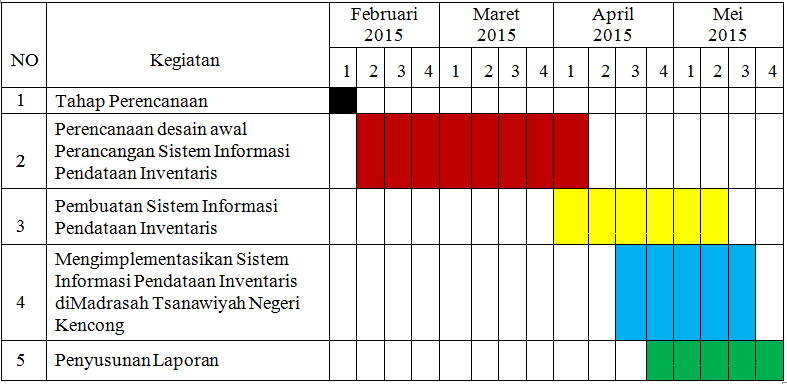
\includegraphics[width=1\textwidth]{gambar/jadwal}
    \caption{Jadwal Penelitian}
    \label{wsn}
\end{table}
\section{Jenis Penelitian}
Dalam penulisan laporan Perancangan Sistem Informasi Pendataan Inventaris ini metode yang digunakan adalah :
\begin{itemize}
\item[1]Studi Pustaka
\\
Data  diperoleh  melalui  buku-buku  dan  tugas  akhir  literature  yang  berhubungan dengan masalah yang akan diteliti sebagai bahan referensi bagi penulis.
\item[2]Teknik Pengumpulan Data
\\
Untuk melakukan riset lapangan diperlukan beberapa teknik pengumpulan   data. Adapun tekniknya yang digunakan adalah :
\begin{itemize}
\item Pengamatan, yaitu pengumpulan data dan informasi yang dilakukan     dengan cara mengamati   langsung   objek   dan   juga   menganalisa   langsung   cara   kerja   proses inventarisasi Madrasah.
\item Wawancara, yaitu pengumpulan data dengan cara melakukan tanya jawab dengan pihak yang terkait di MTs Negeri Kencong sehingga wawancara menghasilkan data yang akurat berdasarkan pendapat staf yang berbeda maka penulis mengambil kesimpulan.
\item Jenis dan Sumber data
\\
Jenis dan sumber data yang digunakan dalam penelitian ini adalah data primer dan skunder. Primer adalah data yang kita dapat langsung dari objek atau  wawancara langsung dengan staf atau pegawai Madrasah yang menangani masalah inventarisasi madrasah. Sekunder adalah data yang tidak langsung atau data yang dapat dari buku-buku dan laporan tugas akhir alumni yang ada di perpustakaan yang relevan dan berhubungan dengan mata kuliah.
\end{itemize}
\item[3]Analisa Sistem
\\
Menganalisis dan mendefinisikan masalah dan kemungkinan solusinya  untuk sistem informasi dan proses organisasi.
\item[4]Perancangan Sistem Database
\\
Merupakan proses untuk menentukan isi dan pengaturan data yang dibutuhkan dalam merancang sistem database yang akan dibuat. Konsultasi dengan dosen pembimbing berkaitan dengan Perancangan  Sistem Informasi pendataan inventaris di MTs Negeri Kencong dan konsultasi mengenai masalah-masalah yang mungkin dihadapi dan solusi penyelesaianya.
\item[5]Implementasi (pengkodean)
\\
Salah  satu  tahap  dalam  membangun  sistem informasi  adalah  implementasi  terdiri  atas koding atau pengkodean yang merupakan tahap menterjemahkan hasil dengan Perancangan  Sistem  Informasi  Inventaris .
\item[6]Pengujian dan Evaluasi
\\
Pada tahap ini, perancangan Sistem telah selesai dibuat dan siap digunakan untuk diuji kebenaranya berdasarkan tujuan pembuatan program.
\item[7]Penyusunan laporan tugas akhir.
\\
Pada tahap  ini  melakukan  pendokumentasian  dalam laporan  dari  seluruh  konsep, dasar teori, implementasi, proses yang telah dilakukan, dan hasil-hasil yang telah didapatkan selama pengerjaan tugas ahir. Laporan tugas akhir ini bertujuan untuk memberikan gambaran dari pengerjaan tugas akhir dan diharapkan dapat berguna untuk pembaca yang tertarik untuk melakukan pengembangan lebih lanjut.

\end{itemize}

\section{Flowchart Sistem}
\begin{figure}[ht!]
  \centering
    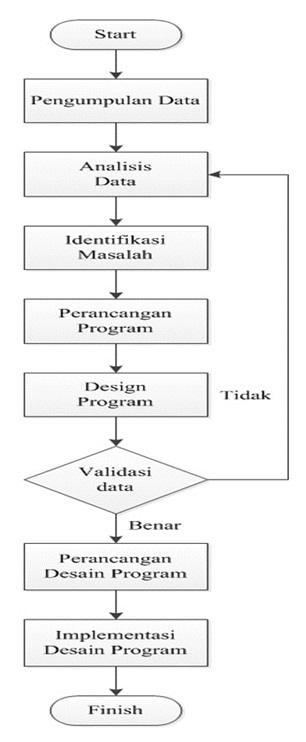
\includegraphics[width=0.5\textwidth]{gambar/flowchart}
    \caption{Gambaran Flowchart Sistem}
    \label{wsn}
\end{figure}
\newpage

\section{Kebutuhan Sistem}
Proses  perancangan  dan  realisasi  perangkat  lunak  Sistem  Aplikasi  Inventaris  ini memerlukan gambar perangkat keras dan lunak sebagai berikut:
\begin{itemize}
\item[1]Perangkat keras
\begin{itemize}
\item Monitor
\item CPU
\item Harddisk  Internal dan Ekternal sebagai media penyimpanan
\item Memori 2 GB
\item Keyboard dan mouse standar
\end{itemize}

\item[2] Perangkat Lunak
\begin{itemize}
\item Sistem operasi window 7
\item Macromedia dreamwaver CS3 sebagai editor dalam bahasa pemograman
\item Xampp server versi .7.7 sebagai server local yang termasuk  didalamnya apache,php dan mysql.
\item Mozilla   firefox   sebagai   browser   dan   tambahan   plugin   yang   membantu menampilkan halaman web.
\end{itemize}
\end{itemize}



\begin{thebibliography}{9}

\bibitem[satu(2015)]{satu01}
Aurino,(2009), ``\textit{Pengenalan Mysql}'', CV. Andi Ofset , Yogyakarta.

\bibitem[dua(2015)]{dua02}
Budi. 2004. \textit{Tehnik Informasi}. Graha lmu, Yogyakarta

\bibitem[tiga(2015)]{tiga03}
Budiono. 2000:2003. \textit{Mengenal Komputer}. CV. Indo Media, Jakarta

\bibitem[empat(2015)]{empat04}
Dwi, Prasetyo, Didik. 2011. \textit{Pemrograman PHP}. PT.Elex Media, Jakarta

\bibitem[lima(2015)]{lima05}
Firdaus, Ir. 2002. \textit{Basis Data}. Informatika Bandung.

\bibitem[enam(2015)]{enam06}
Hendrika. 1991. \textit{Pendataan Barang}. Andi Ofset, Yogyakarta

\bibitem[tujuh(2015)]{tujuh07}
Jefry, Handotyono. 1993. \textit{Jenis Barang-barang}. PT. Erlangga, Bandung

\bibitem[delapan(2015)]{delapan08}
Joianto. 2005. \textit{Sistem Basis Data}. Graha Ilmu, Yogyakarta

\end{thebibliography}
\addcontentsline{toc}{chapter}{DAFTAR PUSTAKA}
%-----------------------------------------------------------------
%Disini akhir masukan Daftar Pustaka
%-----------------------------------------------------------------

\end{document}